\chapter{Planificación y Seguimiento}

En este capítulo detallaramos la planificación de cada una de las iteraciones que hemos hecho, así como el seguimiento realizado. La elaboración de este proyecto se llevó a cabo durante dos años, comenzando en junio de 2014 y teniendo un par de parones durante varios meses (desde septiembre de 2014 hasta enero de 2015 y desde mayo de 2015 hasta septiembre del mismo año). 
Por lo tanto, los periodos de actividad serían los siguientes:

\begin{itemize}
  \item Desde junio del año 2014 hasta septiembre del 2014 (3 meses).
  \item Desde enero de 2015 hasta mayo del mismo año (4 meses).
  \item Desde septiembre del 2015 hasta abril de 2016 (8 meses).
\end{itemize}

En las próximas secciones hablaremos de lo que hemos desarrollado durante estos tres periodos de tiempo y las iteraciones seguidas en los mismos.

Cabe destacar que todos los datos y tareas mostradas a continuación están realizadas de forma lineal, dado que solamente disponemos de un recurso.

\section{Junio 2014 - Septiembre 2014}

Este periodo comienza el 4 de junio, que es cuando se nos comenta la posibilidad de realizar este proyecto, y termina el 24 de septiembre, por lo que consta de un total de 15 semanas. Hay que tener en cuenta que durante parte de este verano (desde agosto) es cuando me mudé a Holanda y empiecé mi \textit{internship}, por lo que las jornadas en días laborables solamente constaban de una o dos horas y alrededor de 8/9 horas durante los fines de semana.

Sumando todo el tiempo empleado durante estas semanas se calcula que se han empleado 190 horas en total.

Durante este tiempo nos centramos en recabar información general para poder empezar el proyecto con buen pie, así como la implementación de los mapas y habitaciones.

\subsection{Primera iteración: Análisis de requisitos generales, diseño genérico y preparación y configuración de los elementos necesarios para el comienzo de la implementación}

Desde el 4 de junio hasta el 29 de junio.

\paragraph{Análisis de requisitos generales} Al desarrollar un proyecto enfocado a una parte de la población de la que no formas parte, es muy importante documentarse sobre todos los aspectos que hay que tener en cuenta e intentar ponerse en su piel (por ejemplo usar las herramientas que utilizan diariamente para recabar ideas).
Àsí mismo, desarrollar un videojuego puede llegar a ser una tarea infinita, dado que nuevas características o ideas que añadir es algo que sucede casi diaremente. Aprender sobre lo básico del género y poner límites es fundamental para centrar los pocos recursos que tenemos en crear lo completamente necesario.

\paragraph{Diseño genérico del juego a implementar} Crearemos el primer diseño genérico que nos dará una idea sobre lo que tendremos que realizar y nos guiará sobre el proceso de creación del juego. Este primer boceto cambiará a medida que querramos añadir nuevos elementos y querramos especificar más otros.

\paragraph{Búsqueda de bibliotecas que se adapten a nuestros requisitos} Hay varias bibliotecas con las que se puede crear una interfaz gráfica sencilla como la de Rogue, pero todas ellas tienen sus ventajas e inconvenientes. Debemos de averiguar cuál de ellas es la más adecuada para nuestro caso.

\paragraph{Creación y configuración del ambiente de desarrollo para poder empezar la implementación} Al empezar un nuevo proyecto debemos de crear un repositorio en git, instalar todo el software necesario y preparar lo básico para que podamos empezar a programar sin encontrarnos con ninguna dificultad a posteriori.

\subsubsection{Tareas y seguimiento}

La descomposición de las tareas es la siguiente:

\begin{enumerate}[label=\bfseries WBS 1.\arabic*]
  \item Análisis de requisitos generales
    \begin{enumerate}[label=\bfseries WBS 1.1.\arabic*]
      \item Estudio de herramientas para invidentes.
      \item Estudio de los elementos del género \textit{roguelike}.
      \item Analizar los elementos encontrados y especificación de lo que queremos en nuestro caso.
    \end{enumerate}
  \item Diseño genérico del juego a implementar.
  \item Búsqueda de bibliotecas que se adapten a nuestros requisitos.
  \item Creación y configuración del ambiente de desarrollo para poder empezar la implementación.
\end{enumerate}

Para la realización de todas estas tareas se planificaron 65 horas en total. Esta estimación se cumplió, por lo que al final de la iteración todas las tareas habían sido realizadas. Ver la figura ~\ref{fig:sec1it1}

\begin{figure}
    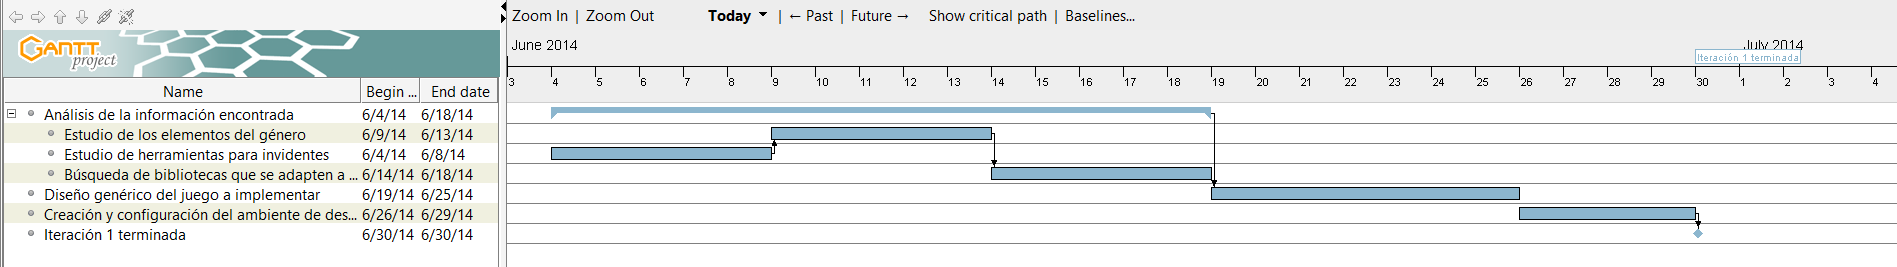
\includegraphics[width=\textwidth,height=\textheight,keepaspectratio]{./img/sec1it1.png}
  \caption{Diagrama de Gantt de la primera iteración de la primera etapa}
  \label{fig:sec1it1}
\end{figure}

\subsection{Segunda iteración: Generación de mapas y habitaciones}

Desde el 15 de julio hasta el 24 de septiembre.

\paragraph{Análisis de requisitos de los mapas y habitaciones} Hay mucho escrito y realizado sobre la creación de mapas y habitaciones de forma aleatoria. En base toda esta información, debemos de elegir lo que queremos realizar en base a, por ejemplo, si el tamaño de dicho mapa siempre será el mismo o no, cómo y cuántas habitaciones queremos tener en cada mapa y el tipo de aletoriedad que queremos (completamente aleatorio o pseudo-aleatorio).

\paragraph{Diseño de los mapas y las habitaciones} Una vez hayamos creado el análisis de requisitos y tengamos toda la información necesaria sobre la mesa, es hora de crear el diseño. Dicho diseño debe de ser fácilmente extendible para que la realización de pequeños cambios no sean un gran reto.

\paragraph{Creación de tests que cubran lo analizado} Tal y como comentamos anteriormente, antes de ponernos con la programación, crearemos los tests que especifiquen y cumplan lo diseñado para, posteriormente, empezar con la codificación.

\paragraph{Implementación del diseño de mapas y habitaciones} Con el diseño y los tests creados, es hora de la implementación del código analizado y diseñado.

\subsubsection{Tareas y seguimiento}

La descomposición de las tareas es la siguiente:

\begin{enumerate}[label=\bfseries WBS 2.\arabic*]
  \item Análisis de requisitos de los mapas y habitaciones.
    \begin{enumerate}[label=\bfseries WBS 2.1.\arabic*]
      \item Estudio de diferentes algoritmos de creación aleatoria de mapas y habitaciones.
      \item Decisión sobre la estructura y tamaño a elegir en base al tipo del juego.
    \end{enumerate}
  \item Diseño de los mapas y las habitaciones.
  \item Creación de tests que cubran lo analizado.
  \item Implementación del diseño de mapas y habitaciones.
\end{enumerate}

Para la realización de esta segunda iteración se planificaron 125 horas en total. La estimación fue correcta y fue posible cumplirla. Ver la figura ~\ref{fig:sec1it2}

\begin{figure}
    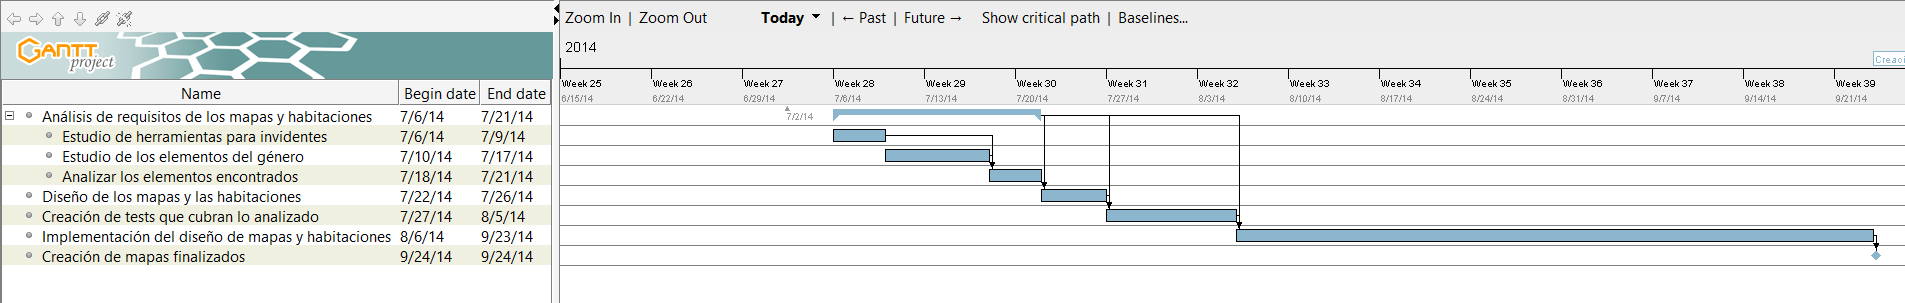
\includegraphics[width=\textwidth,height=\textheight,keepaspectratio]{./img/sec1it2.png}
  \caption{Diagrama de Gantt de la segunda iteración de la primera etapa}
  \label{fig:sec1it2}
\end{figure}

\section{Enero 2015 - Mayo 2015}

Este periodo comienza el 2 de enero, tras los días libres de navidad y nuevo año, y termina el 31 de mayo, en el que pararemos para preparar los exámenes. Por lo tanto, este periodo consta de un total de 21 semanas. Durante estas semanas he estado trabajando a tiempo completo y algunos días se los dediqué a estudiar para los exámenes, por lo que el tiempo semanal empleado fue de alrededor de 12 horas de media, aunque algunas de estas semanas fueron de más trabajo que otras.

En total, 170 horas fueron dedicadas para este sprint inicialmente.

Durante este sprint nos hemos centrado en continuar lo realizado anteriormente y, en general, seguir con el desarrollo del juego en sí.

\subsection{Primera iteración: mapas en IU, análisis, diseño, tests e implementación de los objetos}

Esta primera iteración comienza el 2 de enero y termina el 4 de marzo.

\paragraph{Mostrar los mapas y habitaciones en el interfaz de usuario} En la anterior fase implementamos los mapas, pero no los enseñamos en la interfaz de usuario. En esta ocasión debemos de acabar con esta tarea para terminar con todo lo relacionado con la creación de mapas.

\paragraph{Análisis de requisitos para sobre los objetos} En un \textit{roguelike} los objetos son primordiales. Debemos de investigar qué objetos vamos a usar y cómo los representaremos en el mapa diseñado anteriormente.

\paragraph{Crear un diseño simple sobre cómo los objetos interactuarán con el mapa} Debemos de crear un diseño genérico que nos permita añadir objetos de manera sencilla.

\paragraph{Creación de tests que cubran lo analizado} Al igual que antes, es necesario crear primero los tests en vez de empezar con la implementación del diseño directamente. En este caso también añadiremos tests que interactuen mapas y objetos para asegurarnos que no vamos a tener ningún error cuando combinemos ambos.

\paragraph{Implementación de los objetos en el juego} Una vez realizado el análisis, el diseño y los tests, podremos implementar la solución encontrada.

\subsubsection{Tareas y seguimiento}

La descomposición de las tareas es la siguiente:

\begin{enumerate}[label=\bfseries WBS 1.\arabic*]
  \item Mostrar los mapas y habitaciones en el interfaz de usuario.
  \item Análisis de requisitos sobre los objetos.
    \begin{enumerate}[label=\bfseries WBS 1.1.\arabic*]
      \item Buscar información sobre los diferentes tipos de objetos necesarios en el juego.
      \item Estudiar cómo estos objetos deben de interactuar con el mapa.
      \item Decidir y resumir lo encontrado.
    \end{enumerate}
  \item Crear un diseño simple sobre cómo los objetos interactuarán con el mapa.
  \item Creación de tests que cubran lo analizado.
  \item Implementación de los objetos en el juego y su asociación con el propio mapa y habitaciones.
\end{enumerate}

Para la realización de la primera iteración del segundo bloque de trabajo se planificaron 55 horas en total. La estimación fue correcta y fue posible cumplirla. Ver la figura ~\ref{fig:sec2it1}

\begin{figure}
    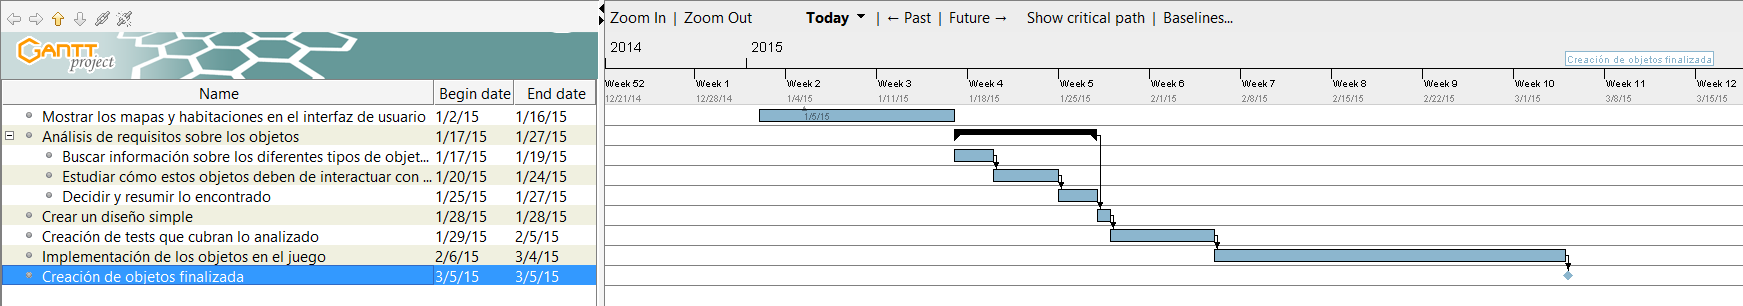
\includegraphics[width=\textwidth,height=\textheight,keepaspectratio]{./img/sec2it1.png}
  \caption{Diagrama de Gantt de la primera iteración de la segunda etapa}
  \label{fig:sec2it1}
\end{figure}

\subsection{Segunda iteración: análisis, diseño, tests e implementación de los personajes}

La segunda iteración comienza el 5 de marzo y acaba el 23 de mayo.

\paragraph{Análisis de requisitos para sobre personajes} En el juego tendremos un personaje principal (controlado por el usuario) y una serie de enemigos con diferentes características que intentarán destruirle y que el usuario deberá de batir. En esta tarea nos encargaremos de buscar información sobre el tipo de enemigos a crear y diferentes métodos para hacerlo de forma más genérica posible, dado que ser capaz de crear estos enemigos fácilmente es una característica fundamental.

\paragraph{Creación del diseño de los personajes} Una vez hayamos realizado el análisis para obtener la idea de los enemigos y personajes a usar, es hora de crear el diseño. Tal y como hemos comentado anteriormente, es necesario hacer un diseño extendible donde crear diferentes clases de enemigos sea lo más sencillo posible.

\paragraph{Implementación de los tests} Como hasta ahora, antes de empezar con la implementación directamente, debemos de crear tests sobre ello, que nos indicará las características que deben de cumplir.

\paragraph{Programación de lo diseñado y analizado previamente} Con el análisis, diseño y tests listos, podremos realizar la tarea de implementación.

\subsubsection{Tareas y seguimiento}

La descomposición de las tareas es la siguiente:

\begin{enumerate}[label=\bfseries WBS 2.\arabic*]
  \item Análisis de requisitos sobre personajes (jugadores y enemigos)
    \begin{enumerate}[label=\bfseries WBS 2.1.\arabic*]
      \item Buscar información sobre los diferentes tipos de enemigos a los que nos enfrentaremos.
      \item Estudiar cómo estos enemigos interectuarán con el mapa y los objetos creados anteriormente.
      \item Decidir y resumir lo encontrado.
    \end{enumerate}
  \item Crear un diseño para crear, fácilmente, nuevos enemigos que aparezcan aleatoriamente en el mapa.
  \item Creación de tests que cubran lo analizado.
  \item Implementación de los enemigos en el juego y su asociación con el propio mapa, habitaciones y objetos.
\end{enumerate}

Para la realización de este \textit{sprint} se han asignado 80 horas, las cuales fueron suficientes para cubrir todo lo que se quiso realizar. Ver la figura ~\ref{fig:sec2it2}

\begin{figure}
    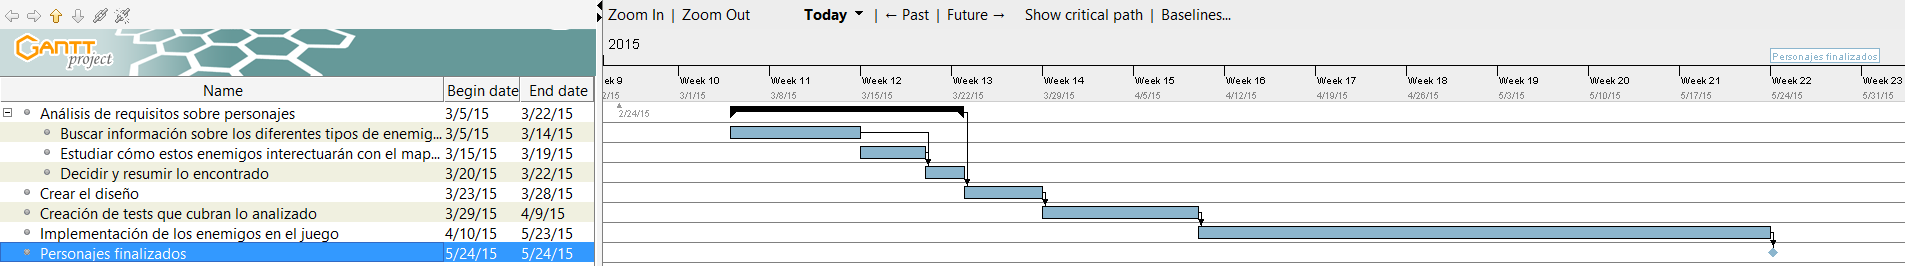
\includegraphics[width=\textwidth,height=\textheight,keepaspectratio]{./img/sec2it2.png}
  \caption{Diagrama de Gantt de la segunda iteración de la segunda etapa}
  \label{fig:sec2it2}
\end{figure}

\subsection{Tercera iteración: interacción entre personajes, tests e implementación}

Esta última iteración de la sección, y la más corta, comienza el 24 de mayo y acaba el 31 del mismo mes.

En la anterior iteración teníamos el objetivo de crear los personajes y enemigos y que éstos fueran capaces de ser representados en la interfaz gráfica. En este caso daremos un paso más allá y deberemos de añadir funciones que dichos personajes puedan realizar con los objetos: creación de un inventario para que puedan almacernarlos y, de tal modo, el usuario y enemigos puedan tener la habilidad de coger objetos (del mapa al inventario), tirarlos (del inventario al mapa), equiparlos (del inventario al personaje) y desequiparlos (del personaje al inventario).

\paragraph{Ampliar los tests sobre la interacción entre los objetos y personajes} En la iteración anterior fuimos capaces de crear los personajes de forma genérica y en este caso deberemos crear nuevas funciones que ayuden a la interacción entre los objetos y los personajes, tal y como hemos descrito anteriormente.

\paragraph{Implementación en base a los tests, análisis y diseño de la anterior iteración} El diseño y el análisis ya lo tenemos hecho y, una vez tengamos los tests creados, podremos realizar la implementación.

\subsubsection{Tareas y seguimiento}

La descomposición de las tareas es la siguiente:

\begin{enumerate}[label=\bfseries WBS 3.\arabic*]
  \item Ampliar los tests que tengan que ver con la interacción entre los objetos y personajes
  \item Implementación en base al diseño de la anterior iteración y los nuevos tests creados.
\end{enumerate}

Al ser un pequeño sprint, hemos sido capaces de terminarlo sin problema. El diagrama de Gantt puede verse en la figura ~\ref{fig:sec2it3}

\section{Enero 2015 - Mayo 2015}